


In this and the next chapter we extend the theoretical work established so far and give it a practical twist to yield two fast approximation algorithms \textsc{Cycle Killer} and \textsc{Nonbinary Cycle Killer}.

Both of these algorithms have two desirable qualities: they terminate quickly even for massive instances of hybridization number and give a non-trivial guarantee of proximity to optimality. These are the first algorithms with such properties. Both algorithms are based on a non-trivial marriage of \maf and \dfvs solvers (both exact and approximate), meaning that further advances in solving \maf and \dfvs will directly lead to improvements in \textsc{Cycle Killer} and \textsc{Nonbinary Cycle Killer}.

This chapter also improves the theoretical work given in the previous one, which also proposed using \dfvs but beginning from a trivial Agreement Forest (AF) known as a \emph{chain forest}. Here we use a smarter starting point: an (approximate) \maf, and it is this insight which makes a 2-approximation (rather than the 6-approximation) possible when using an exact \dfvs solver. Other authors have also had the idea of cycle-breaking in AFs: the advanced FPT algorithm of Whidden et al \cite{whiddenFixed} and the algorithms in the \textsc{HybridNet} family. However, both algorithms start the cycle-breaking from many starting points. In contrast, our algorithm requires only a \emph{single} starting point, i.e. a single (approximate) solution to \maf.

The worst-case running time of both of these approximation algorithms is exponential. However, as we demonstrate with experiments, the running time of our algorithms is in practice extremely fast. For large and/or massively discordant binary trees, \textsc{Cycle Killer} is typically orders of magnitude faster than the \textsc{HybridNet} algorithms and the algorithm in \textsc{Dendroscope}. The performance gap between \textsc{Nonbinary Cycle Killer} and its exact counterparts is less pronounced, but still significant, especially in its fastest mode of operation.

Of course, exact algorithms attempt to compute optimum solutions, whereas our algorithms only give approximate solutions. Nevertheless, our experiments show that when \textsc{Cycle Killer} and \textsc{Nonbinary Cycle Killer} are run in their most accurate mode of operation, an approximation ratio very close to~1 is not unusual, suggesting that the algorithms often produce solutions close to optimality and well within the worst-case approximation guarantee.

The idea behind the binary and nonbinary algorithm is similar. Specifically, we describe an algorithm with approximation ratio ${d(c+1)}$ for the hybridization number problem on two binary trees and an algorithm with approximation ratio ${d(c+3)}$ for the hybridization number problem on two nonbinary trees by combining a $c$-approximation for the problem \maf with a $d$-approximation for the problem \dfvs. Both these problems are NP-hard so polynomial-time algorithms attaining $c=1$ or $d=1$ are not realistic. Nevertheless, there exist extremely fast FPT algorithms for solving \maf on binary trees exactly (i.e. $c=1$), the fastest is \textsc{rSPR} by Whidden, Beiko and Zeh \cite{whiddenRSPRwebsite,whiddenRSPRexp} although the \maf algorithm inside \cite{chen2013ultrafast} is also competitive. Moreover, we observe that the type of \dfvs instances that arise in hybridization practice can easily be solved using Integer Linear Programming (ILP) (and freely-available ILP solver technology such as GLPK), so $d=1$ is also often possible. 

Combining these two exact approaches gives us, in the binary case, an exponential-time approximation algorithm with worst-case approximation ratio~2 that for large instances still runs extremely quickly; this is the \texttt{2-approx} option of \textsc{Cycle Killer}. In practice, we have observed that the upper bound of 2 is often pessimistic, with much better approximation ratios observed in experiments (1.003 on average for the simulations presented in this chapter). We find that this algorithm already allows us to cope with much bigger trees than the \textsc{HybridNet} algorithms or the algorithm in \textsc{Dendroscope}.

Nevertheless, for truly massive trees it is often not feasible to have~${c=1}$. Fortunately there exist linear-time algorithms which achieve $c=3$~\cite{whiddenFixed}. This, coupled with the fact that (even for such trees) it remains feasible to use an exact ($d=1$) solver for \dfvs, means that in practice we achieve a 4-approximation for gigantic binary trees; this is the \texttt{4-approx} option of \textsc{Cycle Killer}. Again, the ratio of 4  is a worst-case bound and we suspect that in practice we are doing better than 4. However, this cannot be experimentally verified due to the lack of good lower bounds for such massive instances. In any case, the main advantage of this option is that it can, without too much effort, cope with trees with hundreds or thousands of taxa and hybridization number of a similar order of magnitude. An implementation of \textsc{Cycle Killer} and accompanying documentation can be downloaded from \url{http://skelk.sdf-eu.org/cyclekiller}. Networks created by the algorithm can be viewed in \textsc{Dendroscope}.

In this chapter we only present the experiments and the theory behind the binary algorithm. The nonbinary case is more involved and we will revisit it in Chapter \ref{ch:3} once the basic idea behind the binary case is clear. 



\section{The algorithm for binary trees}\label{sec:binalg}

We show how \maaf can be approximated by combining algorithms for \maf and \dfvs. In particular, we will prove the following theorem.

\begin{theorem}\label{thm:appr}
If there exists a $c$-approximation for \maf and a $d$-approximation for \dfvs, then there exists a $d(c+1)$-approximation for \maaf (and thus for \mh).
\end{theorem}

%Note that this theorem does not follow from Theorem 2.1 of  \cite{nonbinCK}, since there the approximation ratio for {\sc MAAF} is a $d(c+3)$-approximation. 

To prove the theorem, suppose there exists a $c$-approximation for {\maf}. Let~$T_1$ and~$T_2$ be two trees and let~$M$ be an agreement forest returned by the algorithm. We use notation $\text{\maf}(T_1,T_2)$ and $\text{\maaf}(T_1,T_2)$ for the optimal objective value of a maximum agreement forest and maximum acyclic agreement forest respectively, for input trees $T_1$ and $T_2$. Then,
\begin{equation}\label{eq:mafmaaf}
|M| -1   \leq c \cdot \text{\maf}(T_1,T_2) \leq c\cdot \text{\maaf}(T_1,T_2).
\end{equation}

An $M$-\emph{splitting} is an acyclic agreement forest that can be obtained from~$M$ by removing edges and cleaning up.

\begin{lemma}\label{lem:splitting}
Let~$T_1$ and~$T_2$ be two trees and~$M$ an agreement forest of $T_1$ and~$T_2$. Then, there exists an {$M$-splitting} of size at most $\text{\maaf}(T_1,T_2)+|M|$.
\end{lemma}
\begin{proof}
Consider a maximum acyclic agreement forest~$F$ of~$T_1$ and~$T_2$. For ${i\in\{1,2\}}$, $F$ can be obtained from~$T_i$ by removing a set of edges, say~$E_F^i$, and cleaning up. Moreover, also $M$ can be obtained from~$T_i$ by removing a set of edges, say~$E_M^i$, and cleaning up.

Now consider the forest~$S$ obtained from~$T_1$ by removing $E_M^1\cup E_F^1$ and cleaning up. Then,
\begin{itemize}
\item[$\bullet$] $S$ is an agreement forest of~$T_1$ and~$T_2$ because it can be obtained from~$T_2$ by removing edges $E_M^2\cup E_F^2$ and cleaning up;
\item[$\bullet$] $S$ is acyclic because it can be obtained by removing edges from~$F$, which is acyclic, and cleaning up;
\item[$\bullet$] $S$ can be obtained from~$M$ by removing edges and cleaning up.
\end{itemize}

Hence,~$S$ is an $M$-splitting. Furthermore, $|S| \leq |E_F^1| + |E_M^1| +1$. The lemma follows since $|E_F^1|  = \text{\maaf}(T_1,T_2)$ and $|M|= |E_M^1| +1$.
\end{proof}

Let {OptSplitting$_{T_1,T_2}(M)$} denote the size of a minimum-size $M$-splitting. Combining  Lemma~\ref{lem:splitting} and equation~\eqref{eq:mafmaaf}, we obtain
\begin{equation}\label{eq:mafmaaf2}
\text{OptSplitting}_{T_1,T_2}(M) -1 \leq (c+1) \text{\maaf}(T_1,T_2)
\end{equation}

We will now show how to find an approximation for the problem of finding an optimal $M$-splitting. We do so by reducing the problem to {\sc \dfvs}. We construct an input graph~$D$ for {\sc \dfvs} {(called the \emph{extended inheritance} graph)} as follows. For every vertex of~$M$ that has outdegree 2 (in~$M$), we create a vertex in~$D$. There is an edge in~$D$ from a vertex~$u$ to a vertex~$v$ precisely if in either~$T_1$ or~$T_2$ (or in both) there is a directed path from~$u$ to~$v$. {An example is in Figure~\ref{fig:example}.} We claim the following.

\begin{figure}
  \centerline{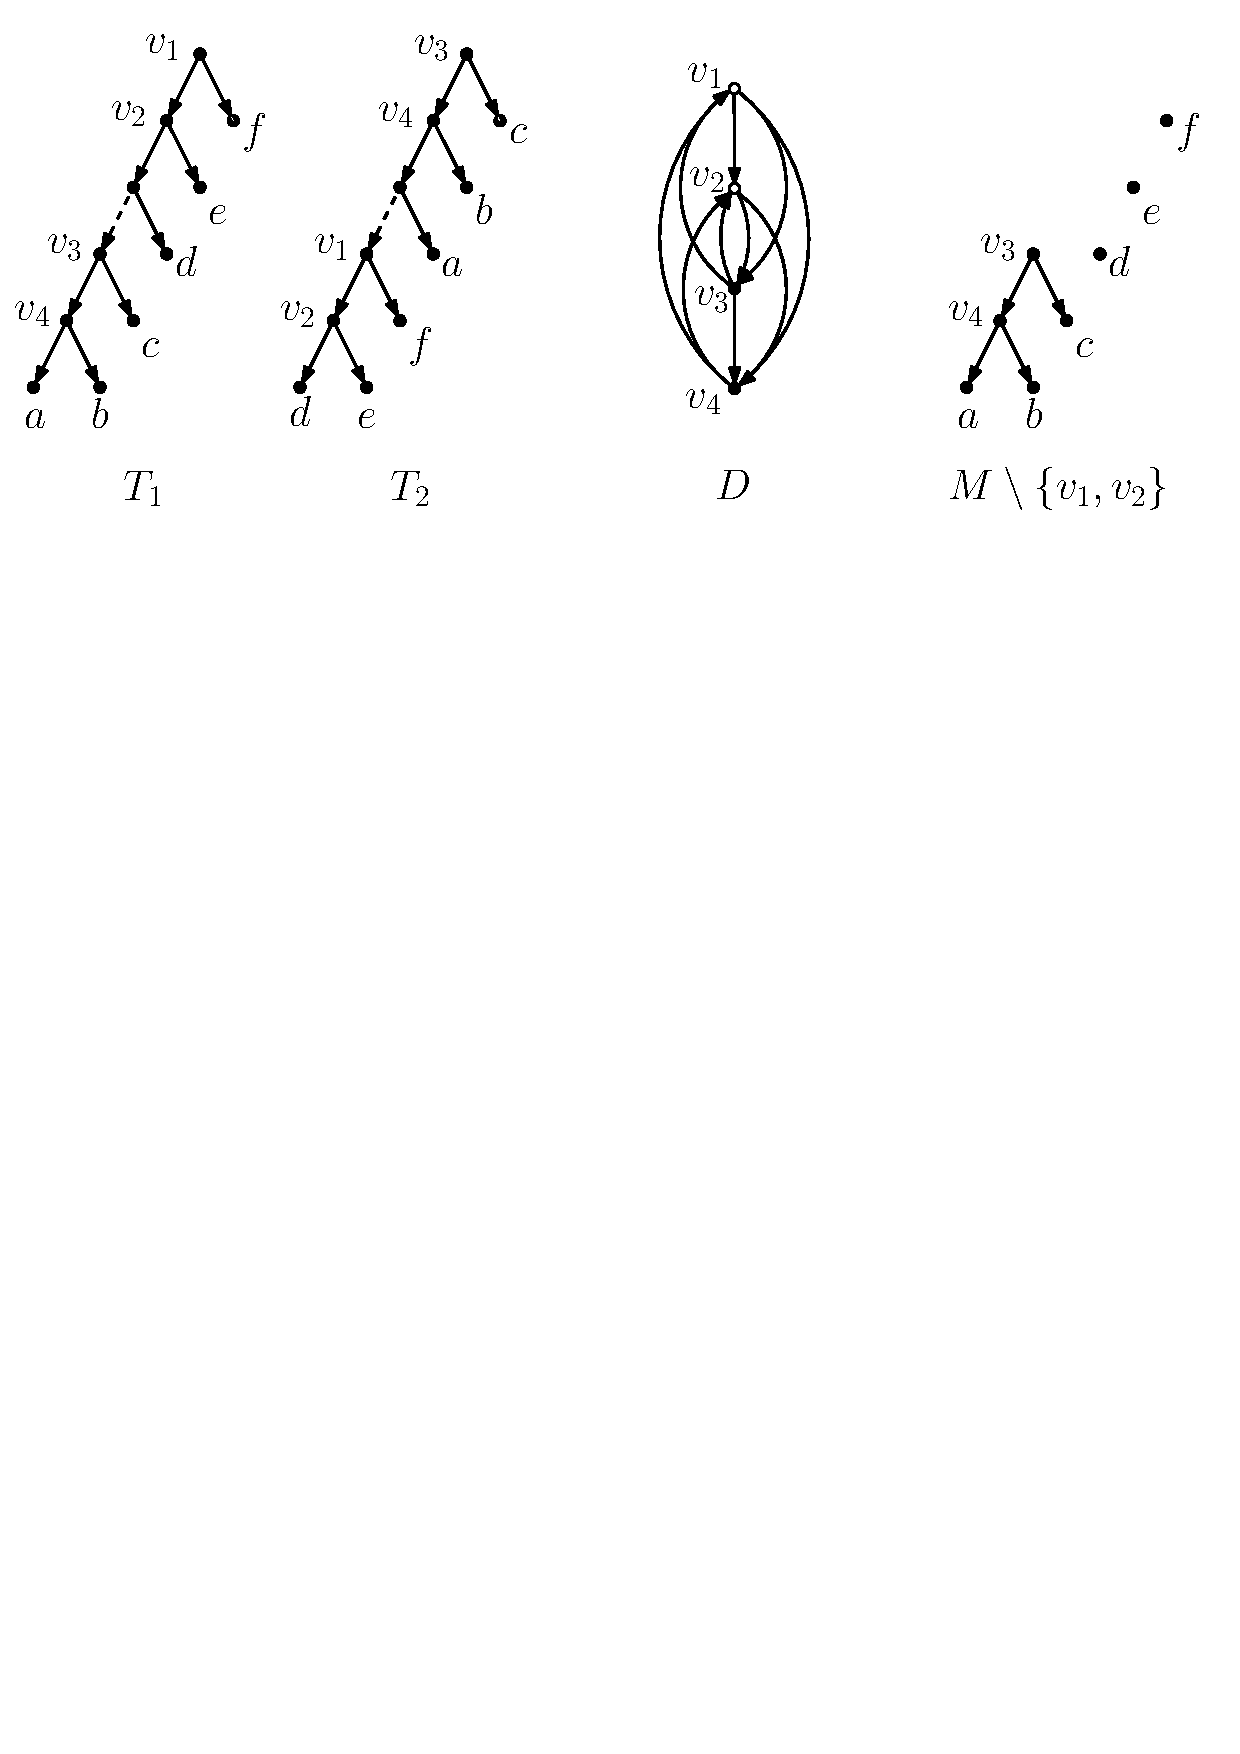
\includegraphics[scale=.6]{../figs/fig_example2}}
  \caption{{Two binary trees~$T_1$ and~$T_2$ and the auxiliary graph~$D$. A maximum agreement forest~$M$ of~$T_1$ and~$T_2$ is obtained by deleting the dashed edges. Graph~$D$ can be made acyclic by deleting either both filled or both unfilled vertices. Hence, removing either~$v_1$ and~$v_2$ or~$v_3$ and~$v_4$ from~$M$ makes it an acyclic agreement forest for~$T_1$ and~$T_2$, see Lemma~\ref{lem:dfvs}. The acyclic agreement forest~$M\setminus\{v_1,v_2\}$ obtained by removing~$v_1$ and~$v_2$ from~$M$ is depicted on the right.}}
  \label{fig:example}
\end{figure}

\begin{lemma}\label{lem:dfvs}
A subset~$V'$ of the vertices of~$D$ is a feedback vertex set of~$D$ if and only if removing~$V'$ from~$M$ makes it an acyclic agreement forest.
\end{lemma}
\begin{proof}
We show that~$D\setminus V'$ has a directed cycle if and only if the inheritance graph of $M\setminus V'$ has a directed cycle.

To prove this, first suppose that there is a cycle $v_1,v_2,\ldots,v_k =
v_1$ in the inheritance graph of $M\setminus V'$. The vertices in the inheritance
graph of $M\setminus V'$ correspond to the roots of the components of $M\setminus V'$. Since these roots have outdegree 2 in $M\setminus V'$, they had outdegree 2 in $M$, and
are thus vertices of $D$. So the vertices $v_1,v_2,\ldots,v_k$ that form the
cycle are vertices of $D$. Since these vertices are in the inheritance
graph of $M\setminus V'$, they can not be in $V'$ and so they are vertices of $D\setminus V'$. The reachability relation between these vertices in $D\setminus V'$ is the same
as in the inheritance graph of $M\setminus V'$. So, the vertices $v_1,v_2,\ldots,v_k$
form a cycle in $D\setminus V'$.

Now suppose that there is a cycle $w_1,w_2,\ldots,w_k = w_1$ in $D\setminus V'$. Each
of the vertices $w_1, w_2,\ldots, w_k$ is a vertex with outdegree-2 in $M$.
Some of them might be roots of components, while others are not.
However, observe that if there is a directed path from a vertex $u$ to a
vertex $v$ in $T_1$ (or in $T_2$) then there is also a directed path from the root of
the component of $M\setminus V'$ that contains $u$ to the root of the component of
$M\setminus V'$ that contains $v$. Hence, there is a directed cycle in the
inheritance graph of $M\setminus V'$, formed by the roots of the components of
$M\setminus V'$ that contain $w_1,w_2,\ldots,w_k$.
\end{proof}

\begin{proof}[{Proof of Theorem \ref{thm:appr}}]
Suppose that there exists a $d$-approximation for {\sc \dfvs}. Let~FVS be a feedback vertex set returned by this algorithm and let~$\text{MFVS}$ be a minimum feedback vertex set. Then, removing the vertices of~$\text{MFVS}$ from~$M$ gives an optimal $M$-splitting. Furthermore, {OptSplitting$_{T_1,T_2}(M) = |M|+|\text{MFVS}|$}. This is because for every vertex in a cycle $C$, its parent in~$M$ must participate in some cycle that contains elements of $C$. So if we start by removing the root of the component we are splitting and subsequently remove only those vertices whose parents have already been removed we see that we add at most one component per vertex. In fact, because vertices of~$D$ all have out-degree~2 in~$M$, we add exactly one component per vertex.

By removing the vertices of~FVS from~$M$, we obtain an acyclic agreement forest~$\cF$ such that
\begin{eqnarray*}
|\cF| - 1 & = & |M| + |\text{FVS}| - 1\\
& \leq & |M| + d\cdot |\text{MFVS}|  - 1\\
& \leq & d (|M| +|\text{MFVS}| - 1)\\
& = & d (\text{OptSplitting}_{T_1,T_2}(M) - 1)\\
& \leq & d (c+1) \text{\maaf}(T_1,T_2),
\end{eqnarray*}
where the last inequality follows from equation~\eqref{eq:mafmaaf2}. Thus,~$\cF$ is a $d(c+1)$-approximation to \maaf, which concludes the proof of Theorem~\ref{thm:appr}.
\end{proof}

{Theorem \ref{thm:appr} implies that a solution to the \maaf problem for a given instance can be constructed by (i)   finding a solution $\mathcal{F}$  to the \maf problem for the same instance  (ii) constructing the  extended inheritance graph $D$ for $\mathcal{F}$ (iii) finding a solution $V$ for the \dfvs problem on the graph $D$ and (iv) modifying $\mathcal{F}$ accordantly to $V$.}



\section{Experiments and discussion}\label{sec:binexp}

To assess the performance of {\sc CycleKiller}, a simulation study was undertaken. We generated 3 synthetic datasets, an \emph{easy}, a \emph{medium} and a \emph{hard} one, containing respectively 800, 640 and 640 pairs of rooted binary phylogenetic trees. 

The easy data set was created by varying  two parameters, namely the number of taxa $n$ and the number of rSPR-moves $k$ used to obtain the
second tree from the first (note that this number is an upper bound on the actual rSPR distance). The 800 pairs of rooted binary phylogenetic trees were created by varying  
$n$ in $\{20,50,100,200\}$ and $k$ in $\{5,10,...,25\}$, and then creating 40 different instances per each combination of parameters.
Each pair $(T_1,T_2)$ of  rooted binary phylogenetic trees for a given set of parameters  $n$ and $k$ is created as follows: 
The first tree $T_1$ on $\mathcal{X}=\{x_1,\dots,x_n\}$ is generated  by first creating a set of  $n$ leaf vertices bijectively labeled by the set $\mathcal{X}$. Then, 
two vertices $u$ and $v$, both with indegree 0, are randomly
picked  and  a new vertex $w$, along with two new edges $(w,u)$ and $(w,v)$, is created. This is done until only one vertex with no ancestor, the root, is present. The  second tree $T_2$ is  obtained from $T_1$ by applying $k$ rSPR-moves.
The medium and the hard data sets were generated in the same way as the easy one, but for different choices of the parameters:   $n$ in $\{50,100,200,300\}$ and $k$ in $\{15,25,40,55\}$ for the medium one and $n$ in $\{100,200,400,500\}$  and $k$ in $\{40,60,80,100\}$ for the hard one.



The exact hybridization number has been computed by \textsc{HybridNet} \cite{hybridnet}, available from \url{http://www.cs.cityu.edu.hk/~lwang/software/Hn/treeComp.html} or with  \textsc{Dendroscope} \cite{Dendroscope3}, available from \url{http://www.dendroscope.org}. We will refer to these algorithms as the \emph{exact algorithms}. Each instance has been run on a single core of an Intel Xeon E5506 processor.

Each  run that took more than one hour was aborted. For each instance, we ran our program with the option \texttt{2-approx}, and, in case the latter did not finish within one hour, we ran it again, this time using the option \texttt{4-approx}, always with a one-hour limit. We used the program \textsc{rSPR} v1.03 \cite{whiddenRSPRwebsite,whiddenRSPRexp} to solve or approximate \maf and GLPK v4.47 (\url{http://www.gnu.org/software/glpk/}) to solve the ILP formulation of \textsc{\dfvs}.

For all instances of the easy data set, {\sc CycleKiller} finished with the \texttt{2-approx} option within the one hour limit, while for 33 instances the exact algorithms were unable to compute the hybridization number. Note that, even for ``easy'' instances, computing the exact hybridization number can take a very long time. To give the reader an idea, for 9 runs of the easy data, \textsc{Dendroscope} and \textsc{HybridNet} did not complete within 10 days. Table~1 shows a summary of the results. It can be seen that {\sc CycleKiller} was much faster than the exact algorithms. Moreover, for 96.6\% of the instances for which an exact algorithm could find a solution, {\sc CycleKiller} also found an optimal solution. While the theoretical worst-case approximation ratio of the \texttt{2-approx} option of {\sc CycleKiller} is~2, in our experiments it performed very close to a 1-approximation.

For the medium data set, {\sc CycleKiller} finished with the \texttt{2-approx} option for 613 instances, and for the remaining ones with the \texttt{4-approx} option. The exact algorithms could compute the hybridization number for only 199 instances (out of 640). For 97.5\% of these instances, {\sc CycleKiller} also found an optimal solution, but with a much better running time.
Regarding the hard data set, 444 runs were completed with the \texttt{2-\hspace{0pt}approx} option and for the remaining ones we were able to use the \texttt{4-approx} option within the given time constraint. Unfortunately, the exact algorithms were unable to compute  the hybridization number for any tree-pair of this data set and hence we could not compute the average approximation ratios.
Over all our experiments, the maximum hybridization number that the exact algorithms could handle was 25.\footnote{In \cite{fastcomputation}, it has been shown that this number can go up to 40 when running Dendroscope on a similar processor but allocating all cores for one instance, i.e. exploiting the possibilities of parallel computation of  this implementation.} In contrast, the \texttt{2-approx} option of {\sc CycleKiller} could be used for instances for which the size of a \maf was up to 97, and thus for instances for which the hybridization number was at least 97.
 
To find the limits of the \texttt{4-approx} option of \textsc{Cycle Killer}, we also tested it on randomly generated trees. On a normal laptop, it could construct networks with up to 10,000 leaves and up to 10,000 reticulations within 10 minutes. Since the number of reticulations found is at most four times the optimal hybridization number, this implies that the \texttt{4-approx} option of \textsc{Cycle Killer} can handle hybridization numbers up to at least 2,500. %These randomly generated trees are, however, biologically meaningless and, therefore, we conducted the extensive experiment described above on trees generated by rSPR moves. Finally we note that over all experiments the worst approximation ratio we encountered was 1.2.

%\textcolor{red}{Interesting things to investigate in future: 1. Implement 3-app algorithm for \maf by BS and see which one performs better on average; 2. For $t$ trees our approach gives a $d(c+1)(t-1)$-approximation because in that case an optimal \maaf is a $(t-1)$-approximation of Hybridization Number, although our implementation only works for two trees. It is currently unclear whether agreement forests can be used to get a better approximation than that.}


\begin{table}\label{table:experiments}
\begin{center}
\begin{tabular}{lr|r|r|r|r|r|r|r|r|}
\cline{3-10}
& & \multicolumn{2}{|c|}{Exact algorithms} & \multicolumn{6}{|c|}{\sc CycleKiller}\\
\hline

 \multicolumn{1}{|l|}{Dataset} & \multicolumn{1}{|l|}{Total} & Com- & \multicolumn{1}{|l|}{Running} &  \multicolumn{2}{|c|}{\texttt{2-approx}}  &  \multicolumn{2}{|c|}{\texttt{4-approx}}&  \multicolumn{1}{|l|}{Average} &  \multicolumn{1}{|l|}{Opt.}\\
 \cline{5-6}
   \cline{7-8}
 \multicolumn{1}{|l|}{} & \multicolumn{1}{|l|}{runs} & \multicolumn{1}{|l|}{pleted} &  \multicolumn{1}{|l|}{time (RT)} & \multicolumn{1}{|l|}{Compl.}  &  \multicolumn{1}{|c|}{RT}  & \multicolumn{1}{|l|}{Compl.}  &  \multicolumn{1}{|c|}{RT} & \multicolumn{1}{|c|}{appr. ratio} &  \multicolumn{1}{|l|}{found}\\
\hline
\multicolumn{1}{|l|}{Easy} & 800 & 767 & 13$m$18$s$ & 800 & 3$s$ & -  & -  & 1.003 & 96.6\% \\
\multicolumn{1}{|l|}{Medium} & 640 & 199 & 42$m$52$s$  & 613  & 3$m$32$s$ & 27 & $<$1 s & 1.002 & 97.5\%\\
\multicolumn{1}{|l|}{Hard} & 640 & 0 & 1$h$ & 440  &  21$m$11$s$ & 200 &1.5 s & - & -\\
\hline
\end{tabular}
\end{center}
\caption{Experimental results. The third column indicates for how many instances at least one exact algorithm finished within one hour. The fifth column indicates for how many instances the \texttt{2-approx} option of {\sc CycleKiller} finished within one hour. For the remaining instances, the \texttt{4-approx} option finished within one hour, as can be seen from the seventh column. The average running time for the \texttt{2-approx} and the \texttt{4-approx} are reported respectively in the sixth and eighth column. The average approximation ratio (ninth column) is taken over all instances for which at least one exact method finished.  The last column indicates the percentage of those instances for which {\sc CycleKiller} found an optimal solution.}
\end{table}
% 
% \section{Conclusion}
% Our experiments with binary trees show that \textsc{Cycle Killer} is much faster than available exact methods once the input trees become sufficiently large and/or discordant. In over $96\%$ of the cases \textsc{Cycle Killer} finds the optimal solution and in the remaining cases it finds a solution very close to the optimum. We have shown that the most accurate mode of the program produces solutions that are at most a factor~2 from the optimum. In practice, the average-case approximation ratio of the most accurate mode that we observed was~1.003. The fastest mode of the algorithm on the other hand can be used on trees with thousands of leaves and provably constructs networks that are at most a factor of~4 from the optimum.
% 
% The central message is: approximating hybridization number by splitting it into \textsc{\maf} and \textsc{\dfvs} instances yields extremely competitive approximation ratios for instances that exact hybridization number solvers will probably never be able to cope with.
